setchapterpreamble[u]{\margintoc}
\chapter{Introduction} 
\labch{intro}

% Importance of multiphase interfacial flows 
\begin{marginfigure}[1cm]
\centering
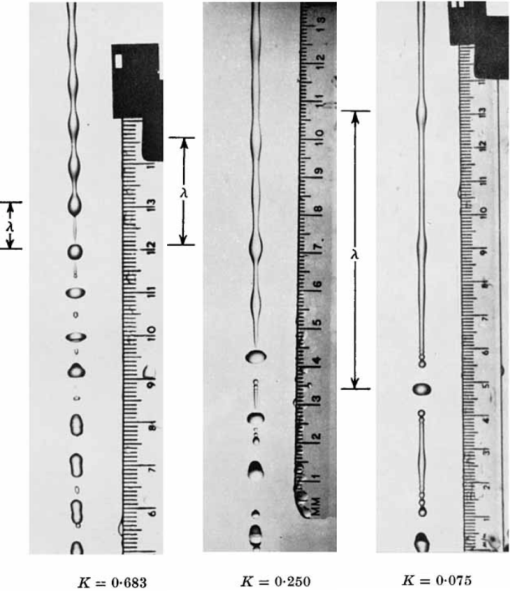
\includegraphics{plots/intro/jet.pdf}
\caption{Decay of a liquid jet into droplets driven by the growth of capillary instabilities corresponding 
	to different excitation frequencies. Image reproduced from Rutland and Jameson \cite{rutland1971non}.
	} 
\label{jet}
\end{marginfigure}

The dynamics of liquid-gas interfacial flows play a critical role in several processes in nature, 
as well as in myriad industrial applications. 
The key elements of surface tension dominated flows such as droplets and bubbles constitute the  
fundamental mechanisms governing the exchange of heat and mass at the ocean-atmosphere interface \cite{seinfeld1998air,deike}, 
mixing/separation in context of metallurgical processes \cite{johansen1988fluid,metal},  
conventional modes of heat transfer \cite{deckwer1980mechanism,bubble}
and ever so importantly, the tranmission of pathogens \cite{lydia_1,lydia_2}. 
One of the most fascinating features of multiphase flows is the process of atomization, 
in which a liquid volume transitions into smaller fragments via a series of topological 
changes of varying complexity, ultimately resulting in the emergence of drops of various sizes
driven by the action of capillary forces at the interface separating the fluids.  
Such processes are ubiquitous in a diverse range of applications spanning from combustion related processes 
(\cite{lefebvre2017atomization,bayvel1993liquid}) to agricultural irrigation (\cite{lake1977effect,reichenberger2007mitigation}).    
In view of the broad spectrum of liquid fragmentation phenomena that pique our scientific interest, 
the present body of work is be divided into two parts :  


\begin{marginfigure}[3cm]
\centering
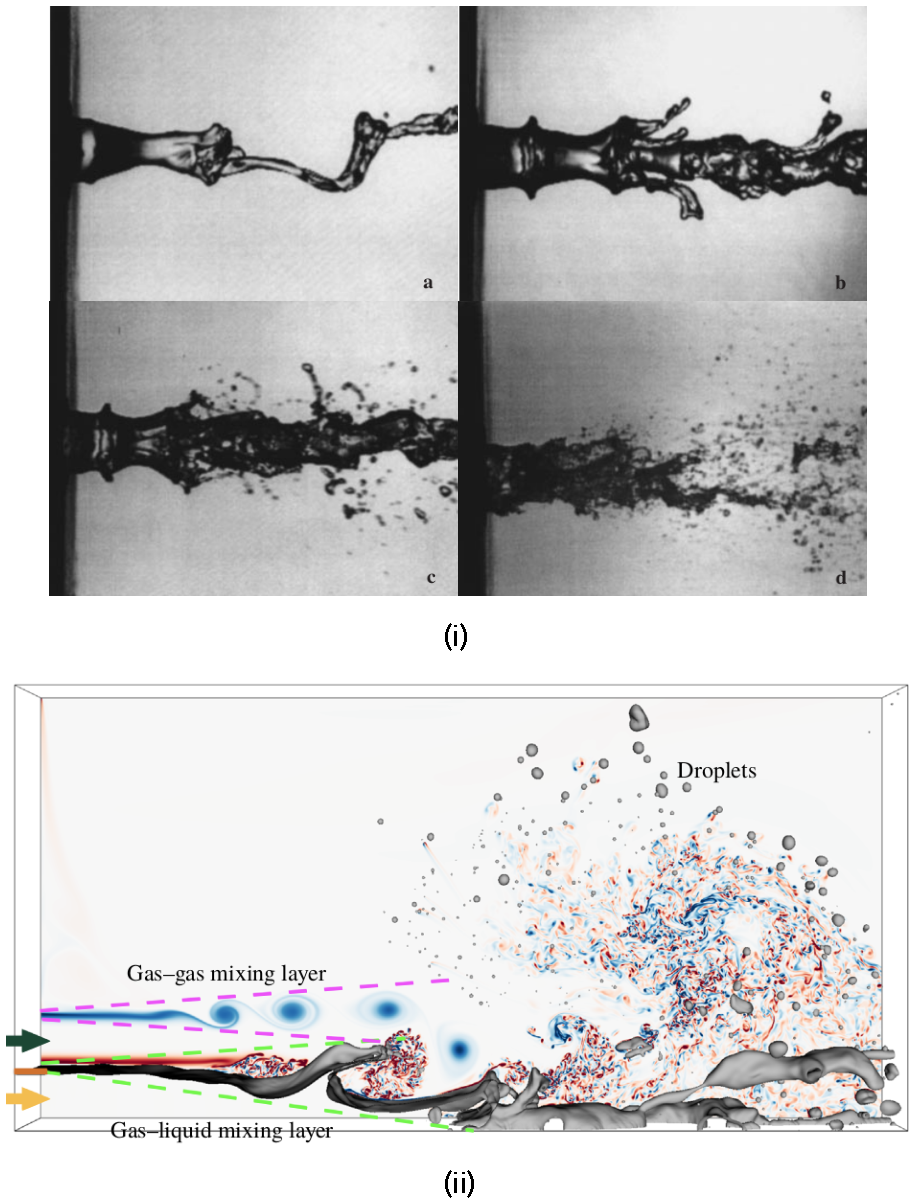
\includegraphics{plots/intro/shear.pdf}
	\caption{ Experimental and numerical investigations of liquid atomization 
	in which the primary stages of topological change are driven by shear instabilities. 
	(i) Liquid jet disintegration by a high speed coaxial gas flow, image reproduced from Lasheras and Hopfinger \cite{lasheras}.
	(ii) Atomization of a two-phase mixing layer between parallel liquid and gas streams, image 
	reproduced from Ling et al. \cite{ling}.
	}
\label{shear}
\end{marginfigure}

% Decay of jets, shear induced atomization, expansion of sheets , hole expansion in sheets, secondary atomization of drops 

\begin{marginfigure}[2cm]
\centering
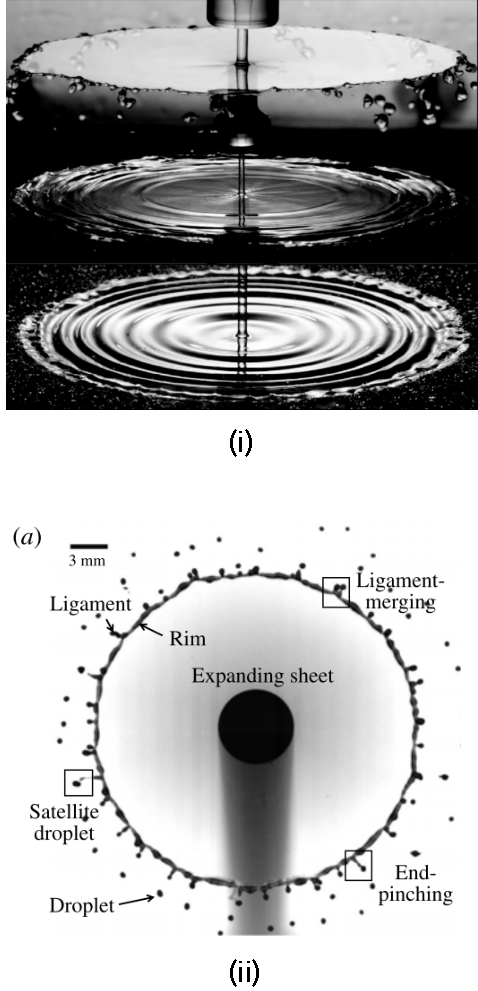
\includegraphics{plots/intro/spread.pdf}
	\caption{ Examples of steady and unsteady liquid fragmentation, demonstrating the disintegration of the  
	radially expanding liquid sheets driven by the capillary deceleration of the rims forming the edges of the sheet. 
	(i) Steady fragmentation of radially expanding sheets driven by jet impact, image reproduced from Bremond et al. \cite{bremond}.
	(ii) Unsteady fragmentation of liquid sheets following drop impact, image reproduced from Wang and Bourouiba \cite{lydia_3}.  
	}
\label{spread}
\end{marginfigure}


\begin{itemize}
	\item Development of numerical methods that can reproduce the dynamics of liquid-gas interfacial flows
		at low to moderate computational cost (spatial resolution), aimed towards flow configurations 
		involving significant contrasts in material properties across the interface. 
	\item Application of numerical methods in an effort to quantify the influence of certain topological
		characteristics of liquid structures on the resulting drop size distributions.  
\end{itemize}

In what follows, we take a closer look at the challenges associated to the above mentioned themes. 

\section*{Challenges in Numerical Modeling}

A substantially large subset of all surface tension dominated flows 
involve significant disparities in the material properties across 
the interface, the most common example being flow configurations 
corresponding to air-water systems, where the densities and viscosities
of the fluids are separated by (approximately) 3 and 2 orders or magnitude, respectively.  
The development of numerical methods that attempt to model 
such interfacial flows involving marked contrasts in density  
face several challenges, key amongst them being the transport of 
mathematical discontinuities that arise out of the aforementioned contrasts. 
Extremely small numerical errors are ubiquitous as a consequence of the 
numerous approximations involved at each and every step of the algorithm
(e.g. propagation of the interface, curvature computation, surface tension modeling etc) . 
In the context of such flows, such ``numerical errors'' may result in physically
inconsistent mass and momentum transfer across the interface, often from
the denser phase towards the lighter phase as a consequence of inadequate numerical resolution.
The presence of large density contrasts tend to amplify
the growth of these cascading numerical errors, eventually
leading to significant (often catastrophic) interfacial deformations
followed rapidly by a loss of numerical stability.

% Artifical Atomization at low resolutions (raindrop crashes).

\begin{marginfigure}[0.5cm]
\centering
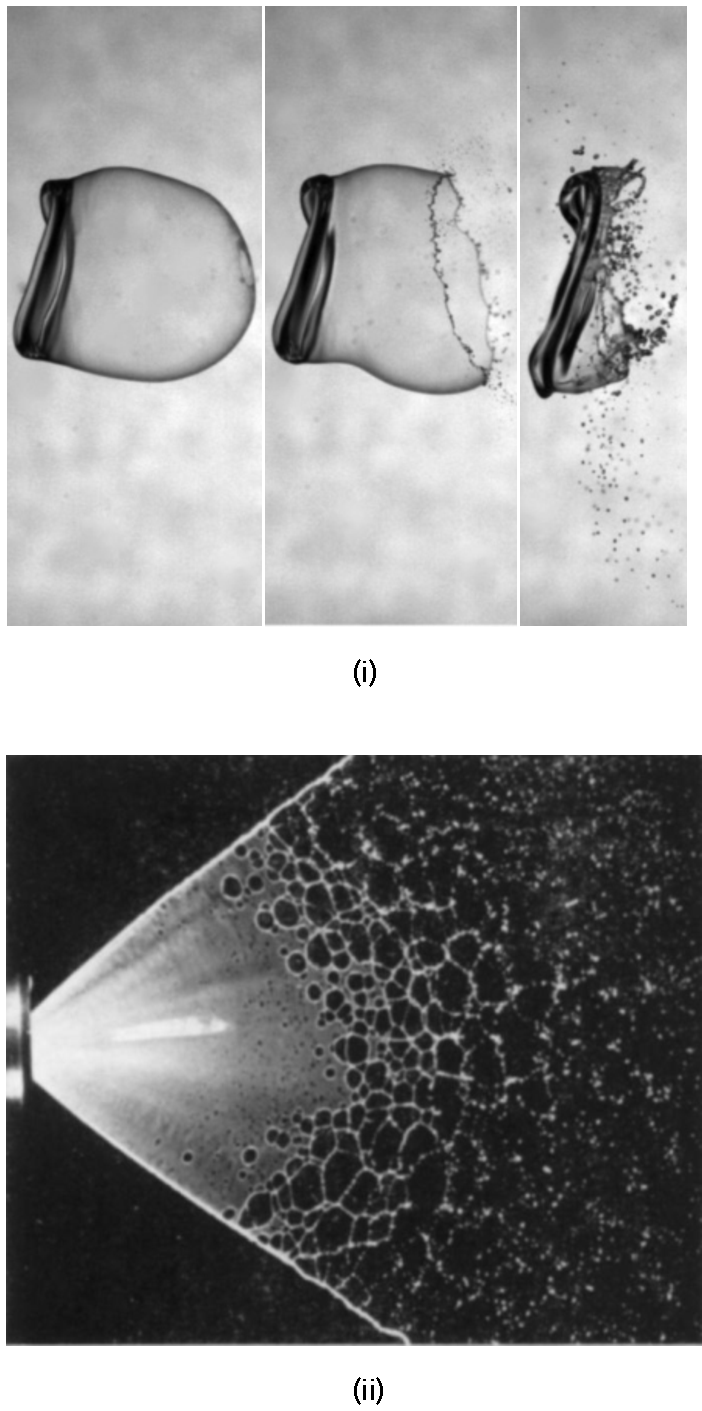
\includegraphics{plots/intro/holes.pdf}
\caption{ Liquid fragmentation triggered by the growth of perforations in thin liquid sheets. 
	(i) Secondary atomization (bag mode) of a drop in a crossflow, driven by the rapid capillary expansion of the hole. 
	Images reproduced from Opfer et al. \cite{hole_drop}.
	(ii) Effervescent atomization of expanding thin liquid sheets driven by the expansion of multiple perforations,
	image reproduced from Dombrowski and Fraser \cite{hole_sheet}.
	}
\label{holes}
\end{marginfigure}


A prime example of such a situation is the numerical simulation of a 
raindrop falling in air under the action of gravity, at speeds near terminal velocity. 
For a regime corresponding to low Weber numbers ($\approx 3$ in our case), there is abundant experimental evidence 
(e.g. see \cite{drop_breakup}) demonstrating that the drops do not undergo any significant deformation, 
apart from some minor shape oscillations driven by the interplay between surface tension and inertia.  
Fig. \ref{explode_compare} shows the results from a moderately resolved numerical simulation, 
where the rapid and uncontrolled growth of numerical errors lead to severe deformations of the interface, 
finally resulting in the un-physical (read ``artificial'') atomization of the raindrop into numerous smaller fragments.


In typical liquid atomization processes, the scale separation
between the sizes corresponding to the largest and smallest liquid structures 
are often several orders of magnitude, which inevitably lead to the smaller 
structures often being poorly resolved due to the inherent limitations in computational power. 
Thus, one can consider that the case of the (less than well resolved) falling raindrop to be 
representative of many of the small structures that emerge out of liquid fragmentation phenomena. 
In that regard, the occurrence of ``artificial'' atomization may significantly distort 
our undertanding of the distribution of drop sizes, as there is no meaningful way 
to distinguish between drops generated via physially consistent processes and 
those produced as a result of cascading numerical errors. 


% demonstrate the effect of such errors, raindrop, 



In the past two decades, considerable efforts have been made 
towards the design of numerical methods to specifically deal with 
flows involving such marked density contrasts
\sidenote{By marked density contrasts, we mean large $|\log r|$, where $r$ 
is the ratio of the densities of the two fluids.}. 
The underlying principle behind these endeavours is that the governing 
equations for the transport of mass and momentum are modeled using a 
conservative formulation (divergence of fluxes), instead of standard 
non-conservative forms which themselves were adapted directly from 
techniques developed originally for single-phase flows. 
This formulation enables one to render the discrete transport of 
momentum \textit{consistent} with respect to the discrete transport of mass.  
Such a tight coupling of the propagation of errors between the discrete 
mass and momentum fields enables alleviation of many of the issues 
that plague such numerical methods, especially in the 
context of low to moderate spatial resolutions (see Fig. \ref{explode_compare}). 


Exacerbating the already complicated nature of the discrete transport of material 
discontinuities is the role of capillary forces on the evolution of the interface. 
They are commmonly modeled as singular source terms in the momentum balance equation that 
governs the evolution of the velocity field, with the capillary force itself 
being proportional to the third derivative of the interfacial position. 
Thus, a secondary but important mitigating factor is the advancements 
made in the modeling of capillary forces, resulting in the adoption of 
consistent and \textit{well-balanced} surface tension formulations.
Consistency in the context of surface tension models refers to the ability 
of methods to progressively achieve more accurate estimations of interfacial 
curvature as a result of increasing spatial resolution, 
whereas well-balanced refers to the ability to recover certain static 
equilibrium solutions pertaining to surface tension dominated flows 
without the perpetual presence of parasitic or spurious currents in the velocity fields.
We refer the reader to influential works of Popinet \cite{popinet2018numerical,popinet2009accurate}
to get a better understanding of the issues surrounding different surface tension implementations.  



% Literature review of different attempts at momcons + summary tables

% Rudman (1998) :
The first study to address the issue of consistency between mass 
and momentum transport was the seminal work of Rudman \sidecite{rudman1998volume}.
The fundamental hurdle in the implementation of mass-momentum 
consistent transport for staggered configurations of primary variables 
(pressure and velocity) is the inherent difficulty in reconstructing mass 
(defined on centered control volumes) and its corresponding fluxes 
onto the staggered control volumes on which momentum is defined. 
Rudman introduced the strategy of carrying out mass advection 
\sidenote{Mass advection was carried out using using algebraic flux reconstructions.} 
on a grid twice as fine as that of momentum, 
thereby enabling a `natural' and intutive 
way to reconstruct mass and its fluxes onto staggered momentum control volumes. 
However, their method uses a VOF based convolution technique for curvature computation, 
which is neither consistent nor well-balanced.    


% Bussmann et al. (2002) :
Bussmann et al. \sidecite{bussmann2002modeling} were able to 
circumvent the issue surrounding staggered grids altogether 
by using a collocated arrangement in the context of hexahedral 
unstructured meshes, coupled with an unsplit Eulerian flux computation method.    
The study though makes no mention of any surface tension model. 


% Raessi & Pitsch (2012) | Ghods & Hermann (2013):
Level set based methods in the context of mass-momentum consistent 
transport were implemented first by Raessi and Pitsch \sidecite{raessi2012consistent}, 
followed by Ghods and Hermann \cite{ghods2013consistent}. 
In the former, the consistency problem is tackled by means of a 
semi-Lagrangian approach, computing geometric level set derived 
fluxes at two different time intervals, whereas in the latter, 
a collocated arrangement is used. 
Nonetheless, both methods face certain drawbacks, notably the 
applicability only to 2D in case of Raessi and Pitsch, 
as well as a lack of well-balanced surface tension models for both these methods.   


% LeChenadec & Pitsch (2013) | Owkes & Desjardins (2017) : 
Recent advances concerning volume-of-fluid based methods that 
employ unsplit (conservative) geometric flux reconstructions 
were made by LeChenadec and Pitsch \sidecite{le2013monotonicity}
, and later by Owkes and Desjardins \cite{owkes2017mass}. 
LeChenadec and Pitsch utilize a Lagrangian remap method in order 
to construct consistent mass-momentum fluxes for the staggered control volumes, 
while Owkes and Desjardins use mass advection on a doubly refined grid 
(same principle as Rudman) to achieve consistency.     
Although \cite{le2013monotonicity} implements a well-balanced surface tension model, 
the VOF convolution based curvature computation is not consistent. 
In case of \sidecite{owkes2017mass}, they use mesh-decoupled height functions 
to compute curvature while coupling it with a well-balanced surface tension model. 
However, their semi-Lagrangian flux computation procedure 
involving streak tubes and flux polyhedra are extremely convoluted in 3D.     


% Vaudor et al. (2017) | Zuzio et al. (2020) : 
Certain methods attempt to combine the qualities of both 
VOF and level set methodologies (CLSVOF), as proposed in the works of 
Vaudor et al. \sidecite{vaudor2017consistent}, 
and more recently by Zuzio et al. \cite{zuzio2020new}. 
They both tackle the consistency issue by means of projecting 
the direction-split geometric fluxes onto a twice finer grid, 
which are subsequently recombined to reconstruct consistent 
fluxes for mass and momentum for the staggered control volumes. 
This approach allows them to bypass the requirement of conducting 
mass advection on a twice finer grid (as in the original Rudman method), 
thereby deriving the benefits of a sub grid without the 
added computational cost of doubly refined mass transport. 
In addition, both Vaudor et al. \cite{vaudor2017consistent} and 
Zuzio et al. \sidecite{zuzio2020new} adopt well-balanced surface tension 
models with consistent level set based curvature estimation. 
However, the purported advantages of both these methods with 
regard to reduced computational costs is not quite evident, 
as additional complexities are introduced due to the projection 
(reconstruction) of fluxes onto a the twice finer mesh, 
which would not be necessary in the first place if mass transport 
had been carried out on the twice finer mesh itself. 


% Patel & Natarajan (2017) : 
Patel and Natarajan \sidecite{patel2017novel} developed a hybrid 
staggered-collocated approach to solve the consistency issue on 
polygonal unstructured meshes, complemented with a well-balanced surface tension model. 
Nevertheless, the VOF advection is based on algebraic transport, 
not to mention the use of a VOF convolution based 
curvature computation, which is inherently not consistent. 


% Nangia et el. (2019) : 
More recently, Nangia et al. \sidecite{nangia2019robust} developed a 
CSLVOF method for dynamically refined staggered Cartesian grids. 
They utilize Cubic Upwind Interpolation (CUI) schemes to 
reconstruct consistent mass and momentum fluxes on the staggered 
control volumes, using the information from the additional mass 
advection equation they solve alongside the level set function.   
However, the reconstruction of mass fluxes using CUI schemes are 
inherently algebraic, with their comparative advantage against fluxes 
computed via geometric constructions being an open question 
\sidenote{refer to Mirjalili et al. \cite{mirjalili2017interface}. }.

To get a bird's eye view of the numerous features employed by the methods 
in existing literature, we refer the reader to tables %\ref{table_vof} and \ref{table_ls}, 
which respectively provide systematic overviews of the VOF based and level set based approaches.    

% Our Approach 

In the present body of work, we start by precisely defining the
essential (desired) attributes of a numerical scheme that 
ensures discrete consistency between mass and momentum transport : 

\begin{itemize}
	\item The discontinuity of the mass (volume fraction 
		derived density field) should propagate at the 
		exact `numerical' speed as that of 
		the discontinuity of the momentum field. 
	\item The numerical transport of momentum should be performed 
		in a manner consistent with the transport of mass for 
		each direction, implying that the momentum fluxes must 
		be obtained directly from geometrically 
		computed fluxes of mass (volume). 
\end{itemize}

\begin{figure*}[h!]
\begin{center}
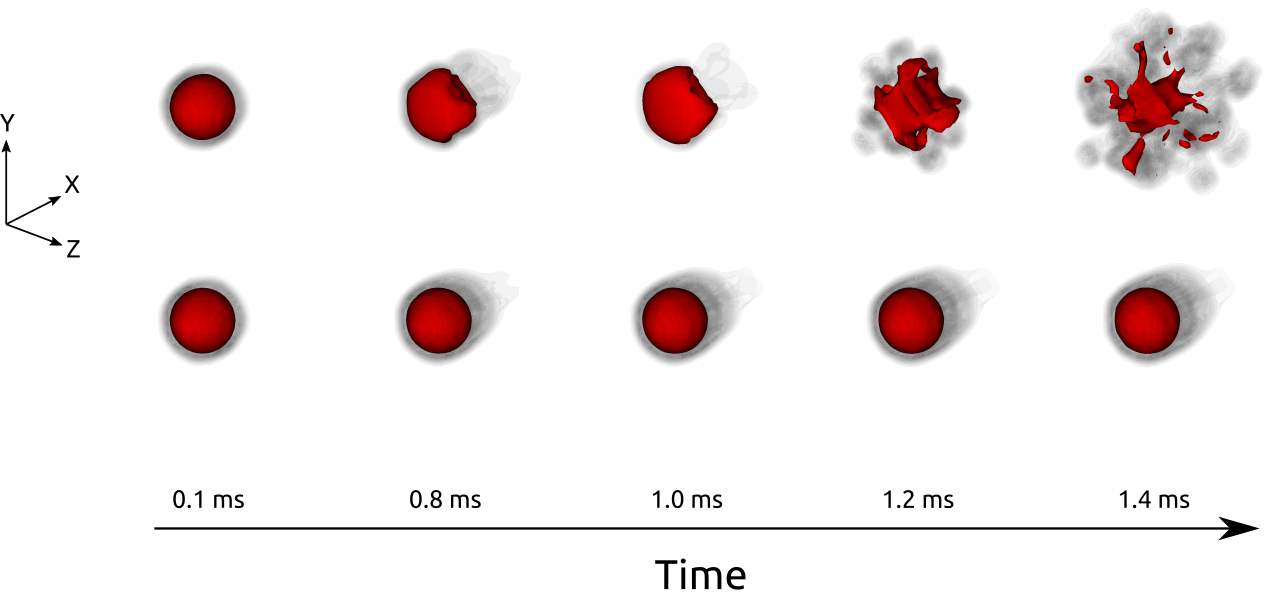
\includegraphics{plots/raindrop/raindrop_explode.png}
\end{center}
\caption{Numerical simulations of a $3 mm$ raindrop falling in air under gravitational acceleration.
	The flow is along the positive X direction, with gravity along the opposite direction. 
	The red contour indicates the isosurface of the volume fraction 
	field corresponding to a value of $0.5$, whereas the black contours 
	surrounding the drop represent isosurfaces of the magnitude of vorticity.
	The droplet has a relatively poor numerical resolution, corresponding to $D/h = 16$,
	where $D$ is the drop diameter and $h$ is the grid size.
	The top row illustrates the phenomenon of ``artificial atomization'' that occurs
	while using the standard version of our numerical method, which does not maintain
	consistency between the discrete transport of mass and momentum.
	In contrast, the implementation of consistent mass and momentum transport
	enables us to supress the massive interfacial deformations of the drop, 
	as evidenced by the bottom row of figures depicting the same flow configuration. 
	The development of methods concerning the consistent transport of mass and momentum 
	is one of the central themes of this study.
	}
	\label{explode_compare}
\end{figure*}

In order to tackle the challenge of consistent transport on staggered control 
\sidenote{`PARIS Simulator' has a staggered configuration of primitive 
variables on regular Cartesian control volumes.}
volume configurations, we have developed two different strategies, namely, 
the \textit{shifted fractions} method and the \textit{sub-grid} method. 
The former uses geometrical reconstructions to derive a 
\textit{shifted} volume fraction field which is centered on the staggered
control volumes, whereas the latter adopts the Rudman \cite{rudman1998volume} 
strategy of volume advection on a twice finer grid in order to 
enable consistent reconstruction of mass and momentum on the staggered control volumes. 
Another key contribution of this body of work is to extend the conservative 
direction-split mass transport algorithm of Weymouth and Yue \sidecite{wy} 
to the direction-split transport of momentum. 

A thorough description of the shifted fractions method is can be found in
the recent study \sidecite{caf_momcons} , and a detailed exposition of the sub grid method 
is currently under preparation at the time of writing.  
We shall be taking a closer look at these two stratetgies in the subsequent chapters.  

\section*{Ligament Mediated Paradigm}

Liquid atomization is basically the transformation of a compact volume into drops.
However, this simplistic view masks the intricate interplay between inertia, viscosity and capillarity across 
different length and time scales spanning several orders of magnitude.  
Such non-trivial interactions are responsible for the abundant variety in the sequence 
of toplogical progressions that eventually lead to the formation of stable drops. 
The most basic transition involves the breakup of a cylindrical filament structure 
(see Fig. \ref{jet}) at approximately regular intervals, driven primarily by the 
growth of long wavelength perturbations due to capillary forces. 
A slightly more complicated transition involves liquid sheets (refer to Fig. \ref{spread}), 
where the inertial expansion of the sheet is opposed by the capillary deceleration of the edges,
resulting in the formation of liquid rims due to volume accumulation at the edges, 
the subsequent destabilization of which leads to the generation of drops. 
Sticking to the breakup of liquid sheets, another imporant transition involves the  
appearance of perforations or holes (see Fig. \ref{holes}) when the thickness of the sheet reaches a certain limit. 
The ensuing rapid expansion of such perforations due to capillary retraction results in the generation of drops. 
Arguably, the most convoluted route to drop formation in encountered when macroscopic 
liquid structures are subjected to shear-driven instabilities (see Fig. \ref{shear}) that 
arise at the interface due to the differential gas and liquid velocities. 
These primary instabilities of the Kelvin-Helmholtz \cite{khi} variety lead to the creation 
of a plethora of secondary structures, many of them corresponding to the aforementioned 
topologies like filaments, expanding sheets with rims, expanding holes in thin sheets etc amongst numerous others. 

The development of a mechanistic understanding into the origins of polydispersity in the drop sizes  
resulting from such fragmentation phenomena has drawn considerable scientific interest throughout the past few decades.
Numerous investigations (both experimental and numerical) into the statistical description of drop sizes
have lead to the popularization of three distinct classes of probability density functions, 
namely the Log-normal, Gamma and Poisson distributions \cite{vill_1}.  
In terms of physical interpretations, the log-normal model \cite{log_normal} is based on a sequential cascade
of breakups, the Gamma family \cite{vill_2} based on the competing effects of aggregation and coalescence of liquid volumes, 
and the Poisson model \cite{poisson} based on the instantaneous and random splitting of a volume into smaller constituents.  
Even though the aforementioned models have been applied to a wide variety of flow configurations
to varying degrees of success, there is a general lack of consensus regarding their validity, primarily 
due to the markedly different trajectories \sidenote{Refer to Wang and Bourouiba \cite{lydia_3} for a discussion.} 
followed by the initial liquid structures towards eventual drop formation. 
Nevertheless, the one common feature that unites these seemingly disparate 
fragmentation processes we have encountered thus far is the transformation 
of the initial liquid topology into transient columnar structures called ligaments. 
It is the evolution and concomitant disintegration of these ligaments 
that finally lead to the production of drops, therefore we entertain 
the possibility that the dynamics of such structures may provide us with 
a universal mechanism that can explain the polidispersity in drop sizes. 


The topological change from the thread-like structure of the ligaments to the 
(approximately) spherical geometry of drops can proceed along different paths, 
depending on whether the drop forms at the free ends or through the 
rupture of the main liquid column at different locations. 
The former mode is referred to as end-pinching \cite{end_pinch_1,end_pinch_2}, 
which generally occurs for regimes ($Oh < O(10^{-2})$) where the capillary driven
retraction of the ligament tips cannot be rapidly damped by the viscous forces. 
Additionally, if the ligament is free at both ends and not slender enough (small elongation ratios), 
there is a possibility that the capillary retraction contracts the entire volume into a single drop \cite{stone_1}. 
The dynamics of the end-pinching mode is further complicated by the interaction of 
additional parameters such as the properties of the surrounding fluid and rate of intertial stretching. 
Despite the richness in the dynamics of end-pinching, the mechanism determining the size of the resulting
drops is quite well understood, with robust scaling laws establishing the drop diameters to be a linear
function of the width of the original ligament \cite{end_pinch_1} (although there is some weak ($We^{-1/7}$) 
dependence on the inertial stretching rate \cite{end_pinch_3} ).  
This turns our attention solely towards the destabilization of the liquid bulk of the ligament. 
The fluid flow in the vicinity of the points of breakup along the liquid thread 
are essentially governed by self-similar solutions \cite{eggers1997nonlinear}, whose local nature 
(independent of initial conditions) is attributed to the intrinsic non-linearities of the Navier-Stokes equations.  
The exact form of such solutions depends on the relative strengths of inertia, capillary forces and viscosity
at that particular length scale, which can be succintly characterized using a phase space composed of Weber and Ohnesorge numbers.  




% Summary of parts and chapters in thesis

% modified comparison charts with CAF paper added

%\thispagestyle{empty}
\clearpage
  \begin{landscape}
      \begin{table}[p]
      	\renewcommand\arraystretch{3.5}
      	\raggedleft
	%\caption{Summary of \textbf{Volume-of-Fluid} based mass-momentum consistent advection methods for incompressible flows of immiscible fluids.}
        \label{table_vof}
	  \resizebox{1.0\textwidth}{!}{%
	  \begin{tabular}[t]{ >{\bfseries\raggedright}m{0.15\linewidth} >{\raggedright}m{0.15\linewidth}  >{\raggedright}m{0.15\linewidth}  >{\raggedright}m{0.15\linewidth} >{\raggedright}m{0.15\linewidth} >{\raggedright}m{0.15\linewidth} >{\raggedright\arraybackslash}m{0.15\linewidth} }
      	  	\toprule
		  & Rudman \newline(IJNMF 1998) &  Bussmann et al. \newline (ASME 2002) & LeChenadec \& Pitsch \newline (JCP 2013) & Owkes \& Desjardins \newline (JCP 2017) & Patel \& Natarajan \newline (JCP 2017) & Present Method \\
      	  	\midrule
		  
		  Basic Configuration & 2D Cartesian, \newline staggered & 3D hexahedral unstructured, \newline collocated & 3D Cartesian, \newline staggered & 3D Cartesian, \newline staggered & 3D polygonal unstructured, \newline staggered & 3D Cartesian \newline staggered \\ 

		  Interface Representation & VOF, Piecewise Linear & VOF, Piecewise Linear & VOF, Piecewise Linear & VOF, Piecewise Linear & VOF, none & VOF, Piecewise Linear \\

		  Flux Computation & split, algebraic Flux Corrected Transport, Eulerian  & unsplit, geometric, Eulerian & unsplit, geometric, semi-Lagrangian & unsplit, geometric, semi-Lagrangian & algebraic Cubic Upwind, Eulerian & split, geometric, Eulerian \\

		  Surface Tension & Continuum Surface-Force & not specified & Ghost-Fluid Method, well-balanced & Continuum Surface-Force, well-balanced & Continuum Surface-Force, well-balanced & Continuum Surface-Force, well-balanced \\
      	  	
		  Curvature Estimation & VOF convolution (smoothed) & not specified & VOF convolution (smoothed) & hybrid mesh-decoupled height functions & VOF convolution (smoothed) & hybrid height functions and curve fitting \\

                 Viscous Stresses & explicit, harmonic averaging & not specified & explicit, harmonic averaging & not specified & explicit, harmonic averaging & explicit, arithmetic averaging \\ 
		  
		  Pressure-Poisson Solver & preconditioned multigrid, Gauss-Seidel & not specified & not specified & not specified & preconditioned GMRES, Krylov subspace & preconditioned multigrid, Gauss-Seidel \\


      	  	\bottomrule
	  \end{tabular}}
      \end{table}
  \end{landscape}	


%\thispagestyle{empty}
\clearpage
  \begin{landscape}
      \begin{table}[p]
      	\renewcommand\arraystretch{3.5}
      	\raggedleft
	      \caption{ }
	      \label{table_ls}
        \resizebox{1.0\textwidth}{!}{%
	  \begin{tabular}[t]{ >{\bfseries\raggedright}m{0.20\linewidth} >{\raggedright}m{0.16\linewidth}  >{\raggedright}m{0.16\linewidth} >{\raggedright}m{0.16\linewidth} >{\raggedright}m{0.16\linewidth} >{\raggedright\arraybackslash}m{0.16\linewidth} }
      	  	\toprule
		  & Raessi \& Pitsch \newline (CAF 2012)& Ghods \& Herrmann \newline (Physica Scripta 2013) & Vaudor et al. \newline (CAF 2017)
		  & Nangia et al. \newline (JCP 2019) & Zuzio et al. \newline (JCP 2020) \\
      	  	\midrule

		  Basic Configuration & 2D Cartesian, \newline staggered & 3D hexahedral unstructured, \newline collocated & 3D Cartesian, \newline staggered & 3D Cartesian \newline staggered & 3D Cartesian \newline staggered \\ 

		  Interface Representation & Level Set & Level Set & Coupled Level Set-VOF & Level Set & Coupled Level Set-VOF \\

		  Flux Computation & Level Set derived, semi-Lagrangian & Level Set derived , Eulerian & split, geometric, Eulerian & algebraic Cubic Upwind, Eulerian & split, geometric, Eulerian \\

		  Surface Tension & Ghost-Fluid Method & Continuum Surface-Force & Ghost-Fluid Method, well-balanced & Continuum Surface-Force, well-balanced & Ghost-Fluid Method \\
      	  	
		  Curvature Estimation & Level Set based & Level Set based & Level Set based & Level Set based & Level Set based \\

                 Viscous Stresses & implicit, harmonic averaging & explicit, arithmetic averaging & semi-implicit, harmonic averaging & explicit, arithmetic averaging & explicit, arithmetic averaging \\ 
		  
		  Pressure-Poisson Solver & preconditioned multigrid, Krylov subspace & not specified & preconditioned multigrid, Conjugate Gradient & preconditioned GMRES, Krylov subspace & preconditioned multigrid, Conjugate Gradient \\


      	  	\bottomrule
	  \end{tabular}}
      \end{table}
  \end{landscape}	

















































